\documentclass[a4paper]{article}
%% Table
\usepackage{booktabs}
\usepackage[table,xcdraw]{xcolor}
\usepackage{multirow}
%% Diagrams
\usepackage{tikz}
%% Bold-font in equation
\usepackage{bm}
%% Language and font encodings
\usepackage[english]{babel}
\usepackage[utf8x]{inputenc}
\usepackage[T1]{fontenc}
\usepackage{placeins}
%% Sets page size and margins
\usepackage[a4paper,top=3cm,bottom=2cm,left=3cm,right=3cm,marginparwidth=1.75cm]{geometry}
%% Useful packages
\usepackage{amsmath}
\usepackage{subfigure}
\usepackage{textcomp}
\usepackage{graphicx}
\usepackage[colorinlistoftodos]{todonotes}
\usepackage{subfig}
\usepackage{float}
\usepackage{mathtools}
\DeclarePairedDelimiter\ceil{\lceil}{\rceil}
\DeclarePairedDelimiter\floor{\lfloor}{\rfloor}
\usepackage[colorlinks=true, allcolors=blue]{hyperref}
\usepackage{authblk}
\usepackage{enumitem}
%% Code
\usepackage{listings}

\title{Extracting semantic and quantitative information from Architectural Floor Plans using Deep Learning networks}
\author{Janamejay Joshi}
\author{Junaid Shaikh}
\author{Subhransu Majhi}
\affil{Center for Computational Technologies, Pune}
\setcounter{Maxaffil}{0}
\renewcommand\Affilfont{\itshape\small}
\begin{document}
\maketitle


\begin{abstract}
Architectural floor plans contain a lot of potential information. The information could be semantic in nature (for example, a pixel could be part of a wall, a door, a window, or a certain type of room) or it could be quantitative in nature (for example, the area/perimeter of a room). Deep learning networks have proven to be highly effective in extracting semantic information from images. In this project we aim to extract semantic information from architectural floor plan images using deep learning networks, and then extract quantitative information from the semantic information using heuristic methods. We design a two-branch multi-task deep learning network in which one branch identifies boundary type (wall, door or window) and the other branch identifies room type. Using the prediction of the boundary type branch, we extract quantitative information relevant to the floor plan and its components.
\end{abstract}


\section{Objectives}
Identification of boundaries (walls, doors/windows) and room-types (closets, washrooms/bathrooms, kitchens/living/dining-rooms, bedrooms, halls, balconies, other room-types, background) in an architectural floor plan. We also wish to extract room corner coordinates and/or contours for rectangular floor plans and use them to calculate associated quantitative information like room area etc.


\section{Introduction}
Recognizing floor plan elements in an image requires one to learn semantic information in the floor plan. It isn't a straightforward segmentation problem since floor plans present not only individual elements (like walls, doors, windows), but also how these elements relate to one another and arrange to make up different room types. Traditionally, image processing methods were used to identify walls, doors etc in a floor plan using geometric patterns (like straight lines and arcs) and using heuristics like Hough transforms. But hand-crafting features most certainly is insufficient as it lacks generality to handle diverse conditions (such as curved walls or plans in which doors aren't represented using arcs). Simple segmentation networks aren't fully equipped to solve the problem as they lack spatial context. We use Zhiliang Zeng's\cite{zengpaper} Deep Floor Plan architecture to tackle this problem as it also includes spatial context.


\section{Zeng's Deep Floor Plan architecture}
\subsection{Salient features}
Zeng's Deep Floor Plan architecture focuses on recognizing floor plan elements like boundaries (walls, doors, windows) and room types (closets, bedrooms, kitchen/living-room/dining-room, hall, bathroom/washroom, balcony). The approach first models a hierarchy of labels for the floor plan elements as shown in Figure \ref{hierarchy}. A multi-task neural network based on the floor plan elements' hierarchy was designed. This network contains a spatial-contextual module to explore the spatial relationship between the elements. The spatial-contextual module is guided by the boundaries (walls, doors, windows) identifying branch of the neural network; i.e. it uses the features learned for the boundaries branch to refine the features learned for the room-type branch. Since the network branches out into two parts, loss functions were designed for both the boundaries identifying branch and the room type identifying branch. A function was also designed to calculate aggregate loss. Thus, the architecture can effectively explore the spatial relationships between the floor plan elements.One of the salient features of the architecture is that it can also handle non-rectangular rooms and walls of non-uniform thickness. 
\begin{figure}[H]
    \centering
    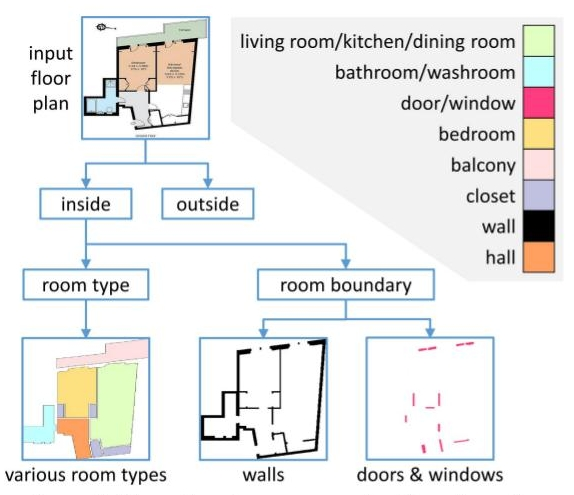
\includegraphics[width=10cm]{hierarchy.jpeg}
    \caption{Hierarchical organization of floor plan elements}
    \label{hierarchy}
\end{figure}
\subsection{Network architecture}
The deep multi-task neural network starts off with a VGG encoder which extracts features from the raw input floor plan image. The features extracted by this VGG encoder architecture are shared for the two subsequent tasks: boundary (walls, doors, windows) prediction and room type (bedroom, hall etc) prediction. The network branches out into two and the shared features are then processed by two separate VGG decoders. This enables the network to learn additional features for each task. Furthermore, each decoding layer in the VGG decoder of the boundaries branch is used to guide the corresponding decoding layer in the VGG decoder of the room type branch. The schematic diagram illustrating the architecture is shown in Figure \ref{archDiag}.
\begin{figure}[H]
    \centering
    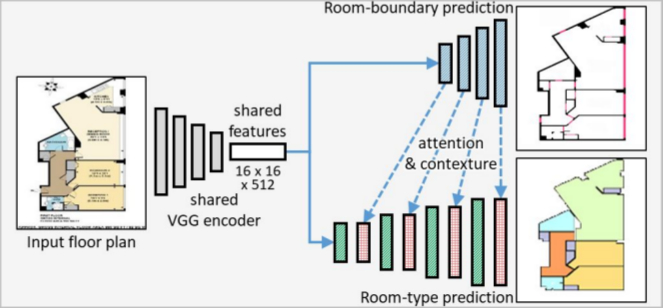
\includegraphics[width=10cm]{architecture.jpeg}
    \caption{Schematic diagram of Zeng's Deep Floor Plan architecture}
    \label{archDiag}
\end{figure}
In Figure \ref{archDiag}, the blue dotted arrows depict the boundary branch VGG decoder layers (blue rectangles) guiding the corresponding room type branch VGG decoder layers (green rectangles) to learn the contextual features (red rectangles). 
The dimensions of features in the network are shown in Figure \ref{layershapes}. The input to the architecture is of shape (\textit{512}x\textit{512}x\textit{3}). The output of the boundaries branch is of shape (\textit{512}x\textit{512}x\textit{3}) and the output of the room type branch is of shape (\textit{512}x\textit{512}x\textit{8}). The three channels in the output of boundaries branch represent background, doors/windows and walls pixels in that order. The eight channels in the output of the room type branch represent closets, washroom/bathroom, kitchen/living/dining-room, bedroom, hall, balcony, others, and background pixels in that order.
\begin{figure}[H]
    \centering
    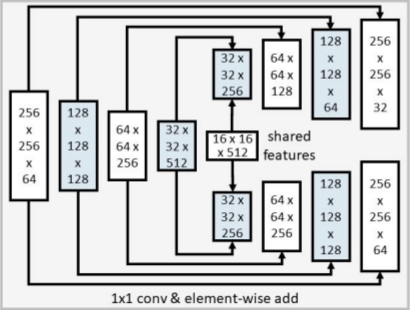
\includegraphics[width=8cm]{layerShapes.jpeg}
    \caption{Dimensions of features in the architecture}
    \label{layershapes}
\end{figure}
The spatial-contextual module helps the room type branch learn contextual features using its VGG decoder layers and the corresponding VGG decoder layer of the boundaries branch. Convolutional layers with four different direction-aware kernels generate features that integrate with attention weights generated from the boundaries branch to produce spatial-contextual features. 
The spatial-contextual module used in Zeng's Deep Floor Plan architecture is shown in Figure \ref{SCM} (where "C" denotes concatenation, and "+" and "x" denote element-wise addition and multiplication respectively). 
\begin{figure}[H]
    \centering
    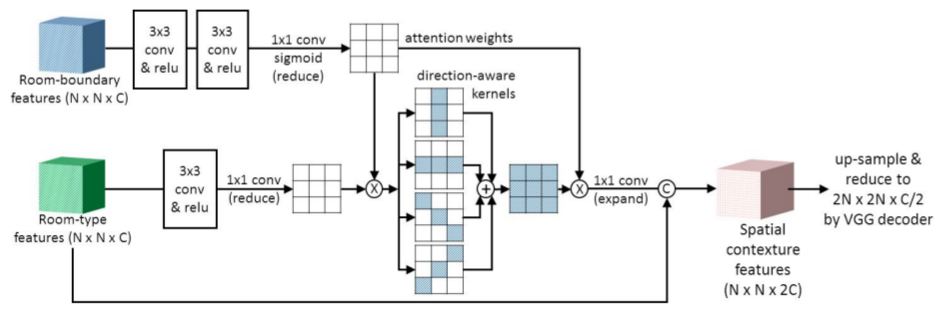
\includegraphics[width=14cm]{spatialcontext.jpeg}
    \caption{Deep Floor Plan architecture's spatial-contextual module}
    \label{SCM}
\end{figure}
\subsection{Losses and Metrics}
We design a within-task weighted loss function to find out the loss for each of the two tasks (boundary and room type identification) and a cross-task weighted loss to find the overall loss across the two tasks. 
\begin{enumerate}
    \item \textbf{Within-task weighted loss}: It is defined in an entropy style as
    \[
    L_{within-task} = w_{i}\sum_{i=1}^{C}-y_{i}\log{p_{i}}
    \]
    where \textit{y$_{i}$} is the label of the \textit{i$^{th}$} floor plan element, \textit{C} is the total number of floor plan elements in the task, \textit{p$_{i}$} is the prediction label for the pixels of the \textit{i$^{th}$} floor plan element. \textit{C} for boundaries branch is 3 (background, doors/windows, walls) and for room type branch is 8 (closets, washroom/bathroom, kitchen/living/dining-room, bedroom, hall, balcony, others, background). \textit{w$_{i}$} is defined as
    \[
    w_{i} = \frac{\hat{N} - \hat{N_{i}}} {\sum_{j=1}^{C}(\hat{N} - \hat{N_{j})}}
    \]
    where \textit{\^N$_{i}$} is the total number of ground-truth pixels for the \textit{i$^{th}$} floor plan element and \textit{\^N}=\sum{$_{j=1}^C$}\textit{\^N$_{j}$}.
    \item \textbf{Cross-task weighted loss}: Let \textit{L$_{bt}$} and \textit{L$_{rt}$} denote the boundary type branch loss and room type branch loss respectively. Let \textit{N$_{bt}$} and \textit{N$_{rt}$} be the total number of network output pixels for boundary type and room type respectively then cross-task weighted loss is defined as
    \[
    L_{cross-task} = w_{bt}L_{bt} + w_{rt}L_{rt}
    \]
    where weights \textit{w$_{bt}$} and \textit{w$_{rt}$} are given by
    \[
    w_{bt} = \frac{N_{rt}}{N_{bt} + N_{rt}}    
    \]
    \[
    w_{rt} = \frac{N_{bt}}{N_{bt} + N_{rt}}
    \]
\end{enumerate}
The outputs of both branches of the network have multiple (\textit{512}x\textit{512}) channels: boundaries branch has 3 (background, doors/windows, walls) and room type branch has 8 (closet, washroom/bathroom, kitchen/living/dining-room, bedroom, hall, balcony, other, background). For measuring the performance of the architecture, we implemented channel-wise accuracy and task-wise accuracy. 
\begin{enumerate}
    \item \textbf{Channel-wise accuracy}: For each channel in the output of a branch of the network, channel-wise accuracy can be calculated as
    \[
    acc_{channel} = \frac{n}{(512 * 512)}
    \]
    where \textit{n} is the number of correctly predicted pixels in the channel.
    \item \textbf{Task-wise accuracy}: For a task of the multi-branch network architecture, task accuracy can be calculated as
    \[
    acc_{task} = \frac{\sum_{j=1}^{m}n_{j}}{m * (512 * 512)}
    \]
    where \textit{m} is the number of channels in task output and \textit{n$_{j}$} is the number of correctly predicted pixels for the \textit{j$^{th}$} channel.
\end{enumerate}


\section{About the dataset}
We used the New York architectural floor plans dataset mentioned in the Zeng's paper, and available on the paper's GitHub repository. The dataset has 179 training images and 53 test images. It contains non-rectangular floor-plans as well. It also provides a walls-annotated image, a doors/windows-annotated image and a room-type-annotated image for each raw floor plan image as shown in Figures \ref{rawData} \ref{walls} \ref{doorsWindows} \ref{rooms}.
\begin{figure}[H]
    \centering
    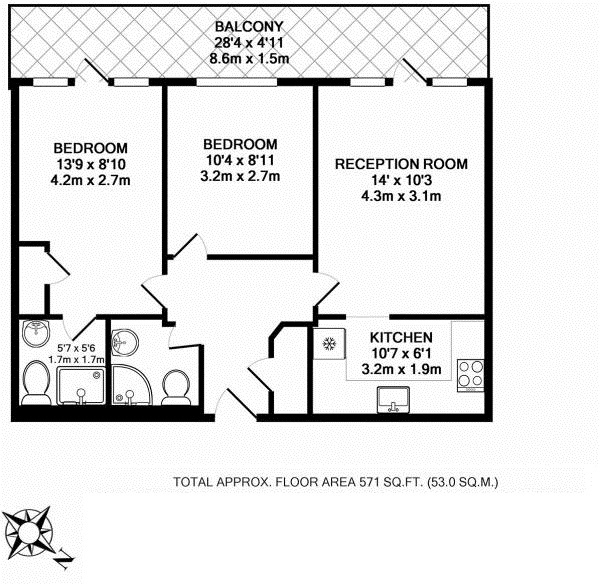
\includegraphics[width=7cm]{raw.jpg}
    \caption{Raw floor plan image from the New York dataset}
    \label{rawData}
\end{figure}
\begin{figure}[H]
    \centering
    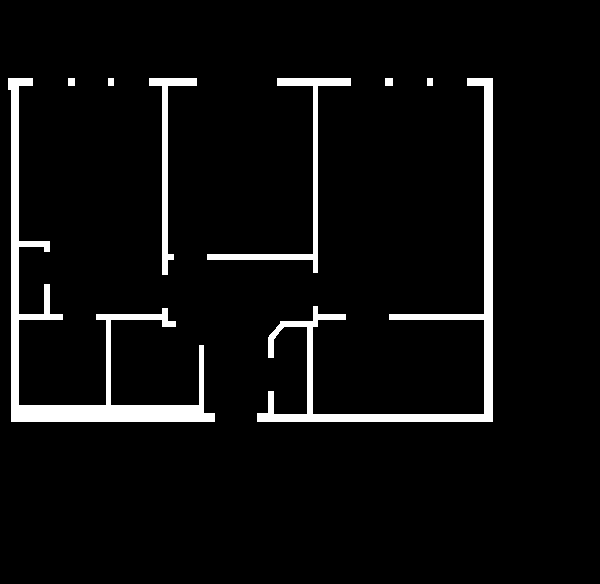
\includegraphics[width=7cm]{wall.png}
    \caption{Walls-annotated image for the raw floor plan image}
    \label{walls}
\end{figure}
\begin{figure}[H]
    \centering
    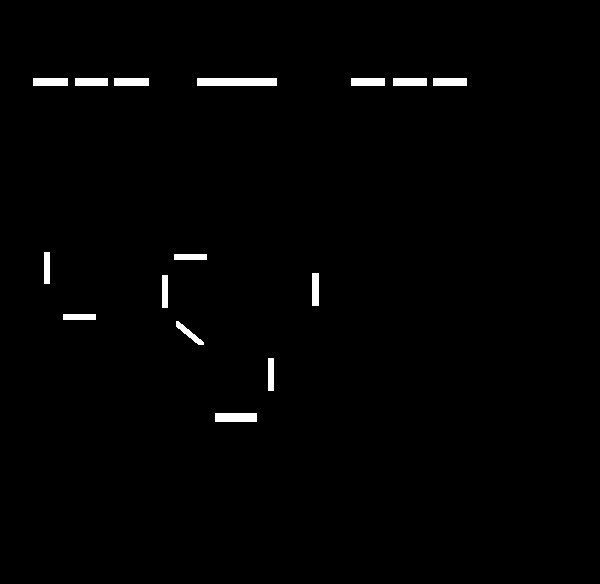
\includegraphics[width=7cm]{dw.png}
    \caption{Doors/windows-annotated image for the raw floor plan image}
    \label{doorsWindows}
\end{figure}
\begin{figure}[H]
    \centering
    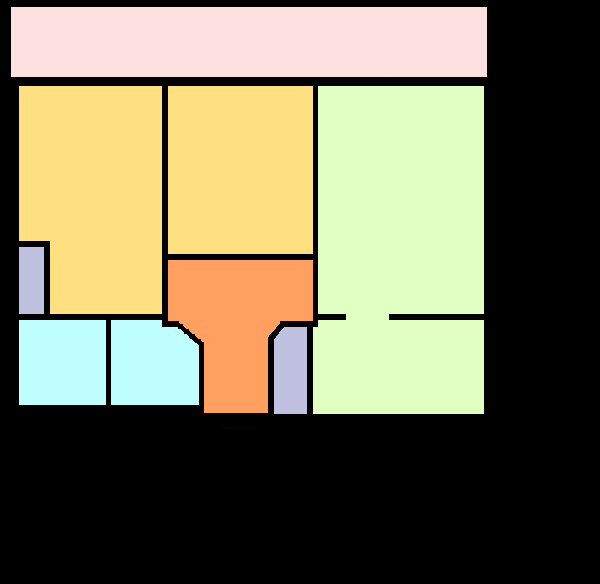
\includegraphics[width=7cm]{room.png}
    \caption{Room-type-annotated image for the raw floor plan image}
    \label{rooms}
\end{figure}


\section{Generating network input and targets}
Since the network takes as input images of dimensions (\textit{512}x\textit{512}), it is important to resize raw floor plan images to those dimensions while maintaining the aspect ratio. Annotated walls, doors/windows and room-type images also need to be resized. Furthermore, since doors/windows and walls are identified by the same branch the their annotated images need to be integrated into a single mask. Since openCV, Tensorflow, Python Image Library (PIL) do not have a resize-with-aspect-ration functionality, an alternate approach is needed. Furthermore, writing a resizing script for the annotated images causes color variations due to interpolation and may add to noise during training. Therefore we designed our own algorithm to resize input images, and target masks for boundaries branch and room-type branch.
\subsection{Resizing input images}
Since slight color variation in input images is harmless, we write a simple resize-image-with aspect ratio script for them. The steps for resizing the input to the architecture are:-
\begin{enumerate}
    \item Convert raw image to array and find array height, width
    \item Create a 3-channel blank white canvas of height and width of 512 pixels each
    \item Find resized image height and width as 
    \[
    newHeight = \floor*{(oldHeight * min(\frac{512}{oldHeight}, \frac{512}{oldWidth})}
    \]
    \[
    newWidth = \floor*{(oldWidth * min(\frac{512}{oldHeight}, \frac{512}{oldWidth})}
    \]
    \item Resize raw image array to \textit{(newHeight, newWidth)} using inbuilt resize functionality with linear interpolation
    \item Relocate resized image array to center of blank canvas
\end{enumerate}
\begin{figure}[H]
    \centering
    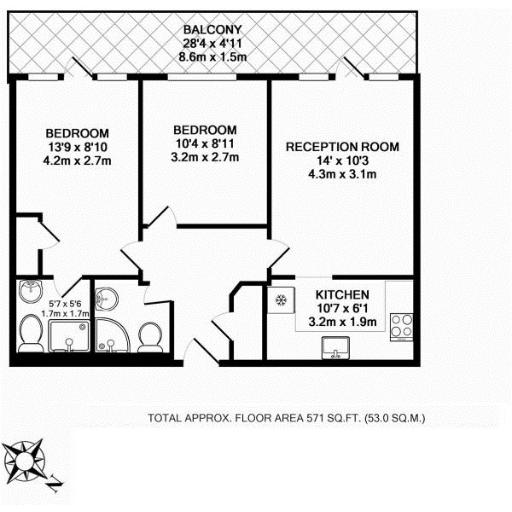
\includegraphics[width=11cm]{53.jpg}
    \caption{Resized-with-aspect-ratio input image for the raw image shown in Figure \ref{rawData}}
    \label{resizedrawData}
\end{figure}
\subsection{Generating boundaries target mask}
We use walls-annotated image and doors/windows-annotated image to create the boundaries target mask. We cannot simply resize the annotated images and combine them as resizing entire images using interpolation causes color variations. Instead we follow the steps given below:-
\begin{enumerate}
    \item From walls-annotated image array, create a single channel binary array of same dimensions: an element in the single channel array has value 1 if the corresponding pixel in the walls-annotated image is a wall pixel, 0 otherwise. Resultant array represents wall channel of original dimensions. We call this array \textit{arr1}
    \item From doors/windows-annotated image array, create a single channel binary array of same dimensions: an element in the single channel array has value 1 if the corresponding pixel in the doors/windows-annotated image is a door/window pixel, 0 otherwise. Resultant array represents doors/windows channel of original dimensions. We call this array \textit{arr2}
    \item From doors/windows-annotated image array, create a single channel binary array of same dimensions: an element in the single channel array has value 1 if the corresponding pixel in the doors/windows-annotated image is a background pixel, 0 otherwise. Resultant array represents background channel of original dimensions. We call this array \textit{arr3}
    \textit Resize \textit{arr3}, \textit{arr2}, \textit{arr1} with aspect ratio, individually, to (\textit{512}x\textit{512}) as described for raw input images.
    \item Stack resized-with-aspect-ratio \textit{arr3}, \textit{arr2}, \textit{arr1} along depth with \textit{arr3} on top.
    \item Handle overlaps between background-doors/windows channels and background-walls channels by assigning them to the corresponding boundaries (doors/windows or walls) channel to obtain the target boundaries mask.
\end{enumerate}
\begin{figure}[H]
    \centering
    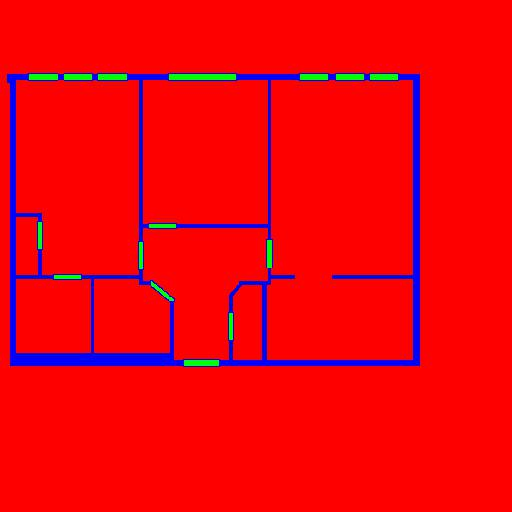
\includegraphics[width=11cm]{boundary.jpg}
    \caption{Target boundaries mask for the resized-with-aspect-ratio raw image shown in Figure \ref{resizedrawData}: Red pixels represent background, Green pixels represent doors/windows, Blue pixels represent walls. Target boundaries mask is of size (\textit{512}x\textit{512}x\textit{3}) and is generated using the annotated-walls image and annotated-doors/windows image}
    \label{boundary}
\end{figure}
\subsection{Generating room-type target mask}
We use the original sized room-type mask to create an 8-channel (\textit{512}x\textit{512}) mask. We use the color encoding used in the original sized room-type mask to do so. Our method of resizing ensures that no color variations occur in the process of resizing.
\begin{enumerate}
    \item For each of the 8 room-types in the original sized room-type mask, we generate a single channel array of the same dimensions: an element of the array has value 1 if the corresponding pixel is of the given room-type, 0 otherwise
    \item We resize each of these single channel binary arrays individually to size {\textit{512}x\textit{512}} as described for raw input images.
    \item We stack the resized single channel binary arrays in the order (closet, washroom/bathroom, kitchen/living/dining-room, bedroom, hall, balcony, other, background) to obtain the (\textit{512}x\textit{512}x\textit{8}) sized room-type target mask.
\end{enumerate}
The color map used to create the RGB format of the 8-channel room-type target map is the same one as used in Zeng's paper. The RGB color map used is: (192,192,224) for closets, (192,255,255) for washrooms/bathrooms, (224,255,192) for kitchens/living/dining-rooms, (255,224,128) for bedrooms, (255,160,96) for halls, (255,224,224) for balconies, (224,224,128) for other room-types, and (0,0,0) for background.
\begin{figure}[H]
    \centering
    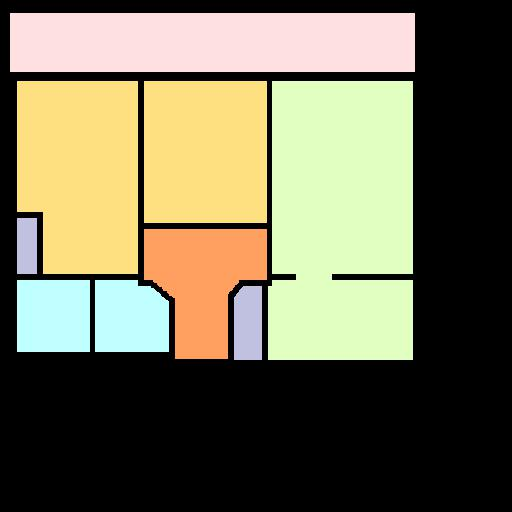
\includegraphics[width=11cm]{53_room.jpg}
    \caption{Target room-type mask in RGB format for the raw image shown in Figure \ref{resizedrawData}. It can be generated using the rooms-annotated image from the dataset. The RGB version of the target mask can be obtained by a color mapping based on which of the 8 channels of the room-type target mask for given pixel coordinates has the value 1. Purple represents closets, cyan represents washroom/bathroom, faint green represents kitchen/living/dining-room, chrome yellow represents bedroom, orange represents hall, pink represents balcony and black represents background}
    \label{roomMask}
\end{figure}


\section{Deep Floor Plan architecture Predictions}
\subsection{Boundaries branch}
We have successfully implemented the upper (boundaries identifying) branch of the Deep Floor Plan architecture. We trained the boundary branch with batch size 1 (like in Zeng's paper) for 204 epochs. The model achieved training accuracy of 70.72\% and testing accuracy of 69.65\%. After epoch 204, the validation loss started to increase and hence training was interrupted. The learning rate for the model varied with the number of epochs:- epoch 1-10: 10$^{-4}$, epoch 11-100: 10$^{-5}$ and after epoch 100: 10$^{-6}$. 
\begin{figure}[H]
    \centering
    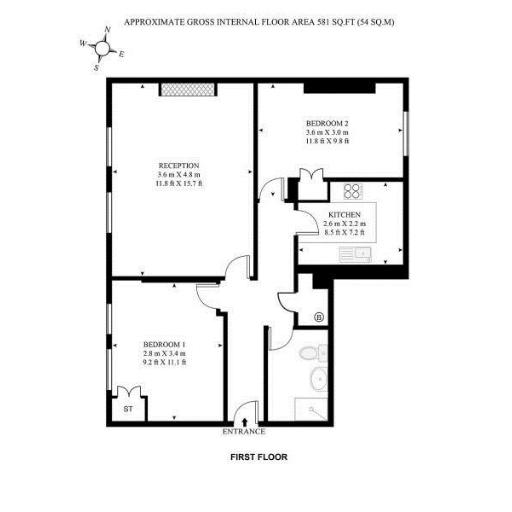
\includegraphics[width=9cm]{testraw.jpg}
    \caption{An example raw input image from the test data}
    \label{testraw}
\end{figure}
\begin{figure}[H]
    \centering
    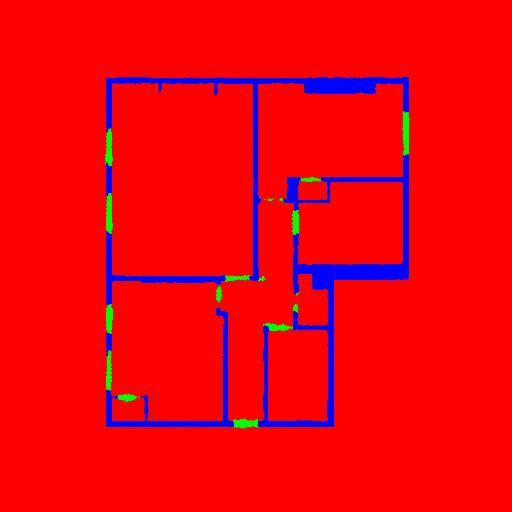
\includegraphics[width=9cm]{testbpred.jpg}
    \caption{Boundaries prediction for the test image shown in Figure \ref{testraw}}
    \label{testbpred}
\end{figure}
\subsection{Deep Floor Plan architecture: Boundaries \& Room-type branches}
We have implemented the full Deep Floor Plan architecture and have also conducted the experiments few times for 2500 epochs. The complete architecture needs fine-tuning and more processing power than is available through Google Colab.


\section{Quantitative information about floor plan image using predictions of Deep Floor Plan architecture}
\subsection{Objectives}
Having obtained the predictions of boundaries (walls, doors/windows) and room-types from the Deep Floor Plan architecture, we use the predictions of the boundaries branch to extract quantitative information about the floor plan. Our primary aim is to extract coordinates of points that make up contours for rooms inside the floor plan and the area enclosed by such contours approximate area of rooms. Related geometric information such as perimeter etc for these contours can also be extracted using our method.
\subsection{Methodology}
\begin{enumerate}
    \item A single channel image is obtained by combining channel2 (doors/windows channel) and channel3 (walls channel) of the prediction of the boundaries branch of the Deep Floor Plan architecture. An example of such an image is shown in Figure \ref{c1c2}.
    \begin{figure}[H]
    \centering
    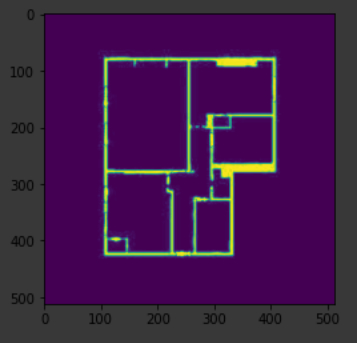
\includegraphics[width=9cm]{c1c2.jpg}
    \caption{Single channel image obtained by combining channel2 (doors/windows) and channel3 (walls) of boundaries prediction image \ref{testbpred}}
    \label{c1c2}
    \end{figure}
    \item This binary image is thinned using openCV's Zhang-Suen thinning algorithm to reduce thickness of boundaries to single pixel. There may be small gaps in the boundaries due to errors in prediction. Steps 3, 4, 5 try to fill such gaps that are small in size. An example of such a thinned image is shown in Figure \ref{c1c2thin}.
    \begin{figure}[H]
    \centering
    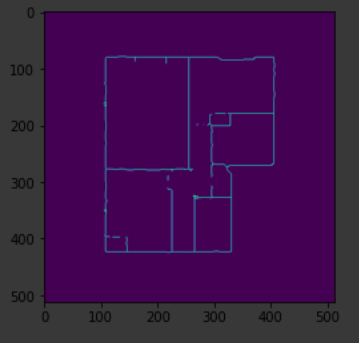
\includegraphics[width=9cm]{c1c2thin.jpg}
    \caption{Single channel image obtained by thinning combined doors/windows and walls channels image shown in Figure \ref{c1c2}. Notice that there are gaps in the boundaries of the thinned image}
    \label{c1c2thin}
    \end{figure}
    \item Invert the thin image and calculate a distance field type mask which measures distance from nearest boundary-type (wall, door/window) pixel. Find maximum distance value in this mask. An example of such a distance-field-type mask is shown in Figure \ref{c1c2dist}.
    \begin{figure}[H]
    \centering
    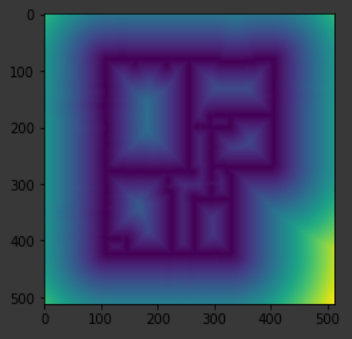
\includegraphics[width=9cm]{c1c2dist.jpg}
    \caption{Distance-field-type mask obtained with respect to distance from boundary-type (walls, doors/windows) pixels of thinned image shown in Figure \ref{c1c2thin}}
    \label{c1c2dist}
    \end{figure}
    \item Identify all pixels in the mask which lie within 6\% of this maximum distance from boundary-type (wall, door/window) pixels. This will lead to the creation of an image with thick boundaries. An example of such a thick-boundaries image is shown in Figure \ref{c1c2thick}.
    \begin{figure}[H]
    \centering
    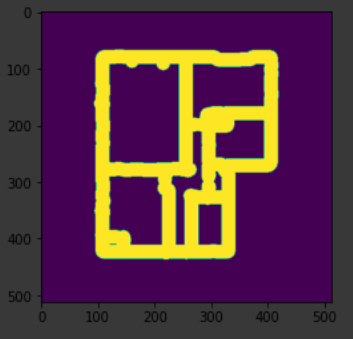
\includegraphics[width=9cm]{c1c2thick.jpg}
    \caption{Thick-boundaries image obtained by finding pixels within 6\% of the maximum distance from the boundary-type pixels. The thick-boundaries image is obtained from the distance-field-type mask shown in Figure \ref{c1c2dist}}
    \label{c1c2thick}
    \end{figure}
    \item Perform skeletonization on this thick boundaries image. It results in an image in which boundaries are thinned and small gaps due to prediction error in the boundaries are filled. An example of such a skeletonized version of a thick-boundaries image is shown in Figure \ref{c1c2skele}.
    \begin{figure}[H]
    \centering
    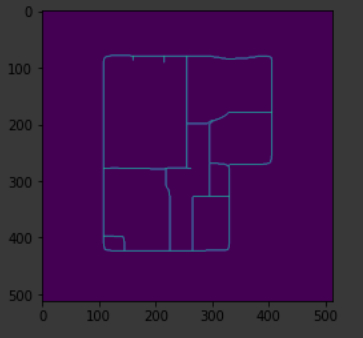
\includegraphics[width=9cm]{c1c2skele.jpg}
    \caption{Single channel image obtained by skeletonizing the thick-boundaries image shown in Figure \ref{c1c2thick}. Notice that the gaps in the boundaries of Figure \ref{c1c2thin} have been filled in. A small closet has been consumed by one of the rooms (One of the shortcomings of our Quantitative Information extraction methodology which we have mentioned later)}
    \label{c1c2skele}
    \end{figure}
    \item Contours in this image can be identified using openCV's findContours functionality and information like perimeter, area and coordinates of points in the contours can also be extracted.
    \begin{figure}[H]
    \centering
    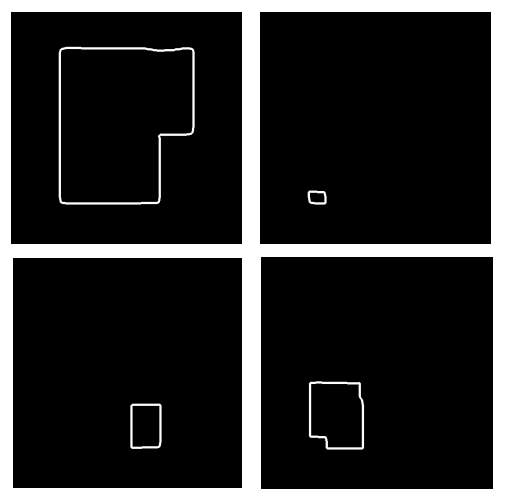
\includegraphics[width=8cm]{cont1.jpg}
    \end{figure}
    \begin{figure}[H]
    \centering
    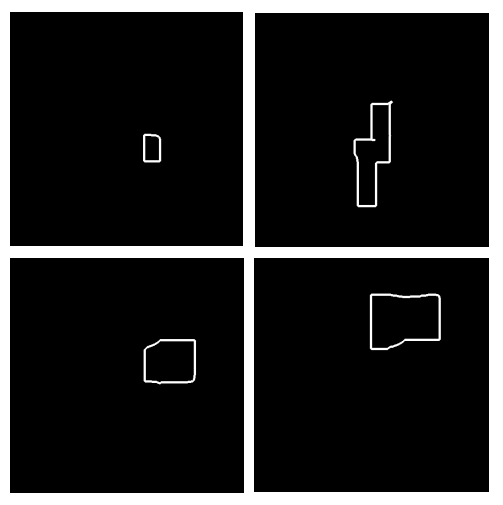
\includegraphics[width=8cm]{cont2.jpg}
    \end{figure}
    \begin{figure}[H]
    \centering
    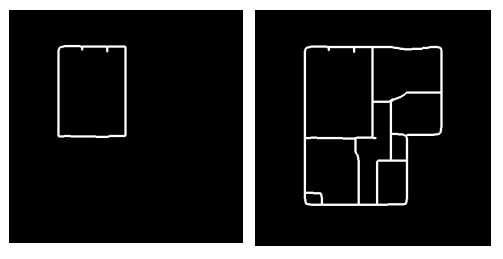
\includegraphics[width=8cm]{cont3.jpg}
    \caption{Contours extracted from the skeletonized image shown in Figure \ref{c1c2skele}. One of the small closets in the floor plan has been consumed completely in a room as a result of the thinning-thickening-skeletonization process}
    \end{figure}
\end{enumerate}
\subsection{Shortcomings of our methodology}
\begin{enumerate}
    \item The 6\% threshold of identifying pixels close to boundary pixels while trying to fill in prediction gaps is set by observation. This may not be effective while trying to fill-in large gaps and may also distort geometry of small rooms.
    \item The contours that are using openCV's findContours functionality may not always make sense. For example, for non-rectangular floor plans small sections of arcs in curved walls are identified as contours. Thus contours may not always be closed figures.
    \item Shapes of contours aren't perfectly rectangular but rather are approximations. Hence information like area etc is also an approximation of its actual value. 
\end{enumerate}


\section{Conclusion and future work}
The initial target of the project was to identify boundaries (walls, doors/windows) in a floor plan and extract numerical information related to the floor plan like room-corner coordinates, room area etc. We were successfully able to that using the upper (boundaries identification) branch of Zeng's Deep Floor Plan architecture. Our methodology of extracting quantitative information relevant to floor plan analysis also works well for rectangular floor plans, though it has some shortcomings. 
For future work, the implemented full Deep Floor Plan architecture can be fine-tuned so the task of room-type semantic segmentation can also be performed. 


\bibliographystyle{alpha}
\begin{thebibliography}{99}
\bibitem{zengpaper} Zeng Z., Li X., Yu Y. "Deep Floor Plan Recognition Using a Multi-Task Network with Room-Boundary-Guided Attention" In: ICCV (2019)
\end{thebibliography}
\end{document}